\newcommand{\makeSampleFig}{%
\begin{figure}[tb]
 \centering % avoid the use of \begin{center}...\end{center} and use \centering instead (more compact)
 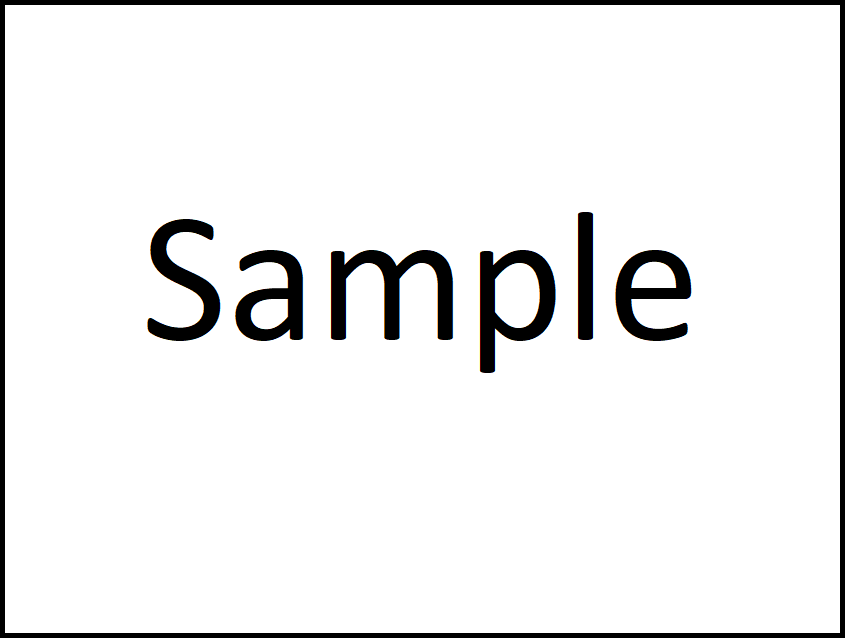
\includegraphics[width=\columnwidth]{sample}
 \caption{A visualization of the 1990--2015 data from \autoref{tab:vis_papers}. The image is from \cite{Isenberg:2017:VMC} and is in the public domain.}
 \label{fig:sample}
\end{figure}}

\newcommand{\makeSampleSegFig}{%
\begin{figure}[!htbp]
    \centering
    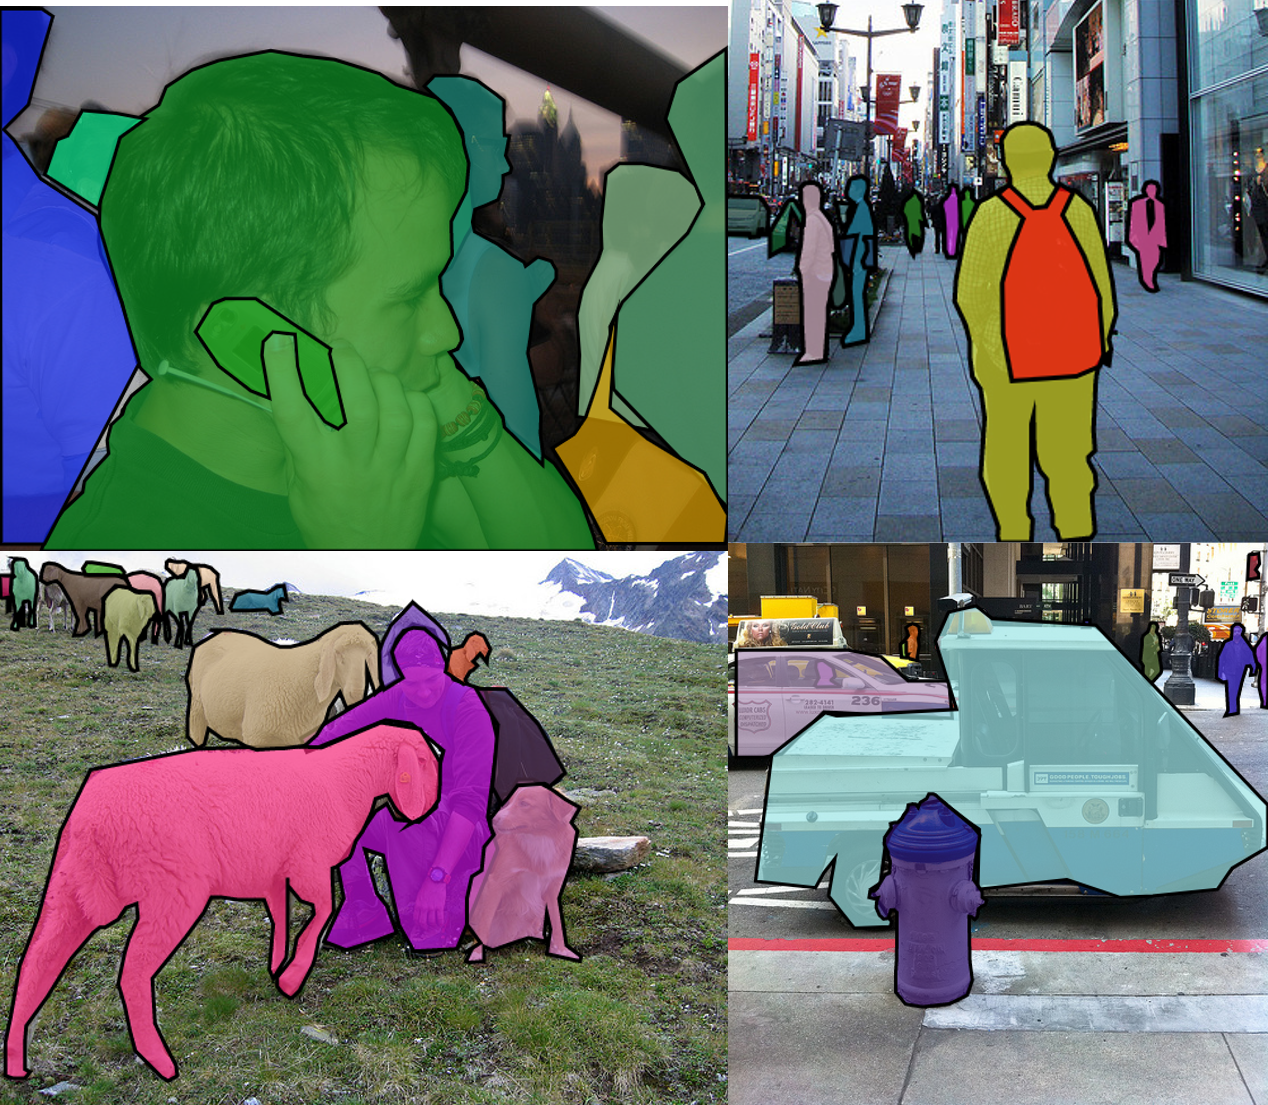
\includegraphics[width=\linewidth]{figures/sampleSegData}
    \caption{Common use cases for semantic segmentation involve relatively few foreground objects, low-resolution data, and limited complexity per object.}
    \label{fig:sampleSegData}
\end{figure}
}

\newcommand{\makeBeesFig}{%
\begin{figure}[!htbp]
    \centering
    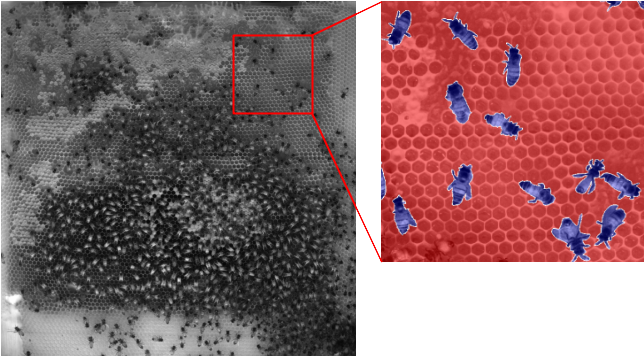
\includegraphics[width=\linewidth]{figures/bees}
    \caption{Sample segmentation involving a high-resolution image with many regions of interest and high foreground complexity.}
    \label{fig:bees}
\end{figure}
}

\newcommand{\makeReconfigFigs}{%
\begin{figure*}[!htbp]
    \centering
    \subfloat[Example using component ID (the default) as a coloring label]{%
        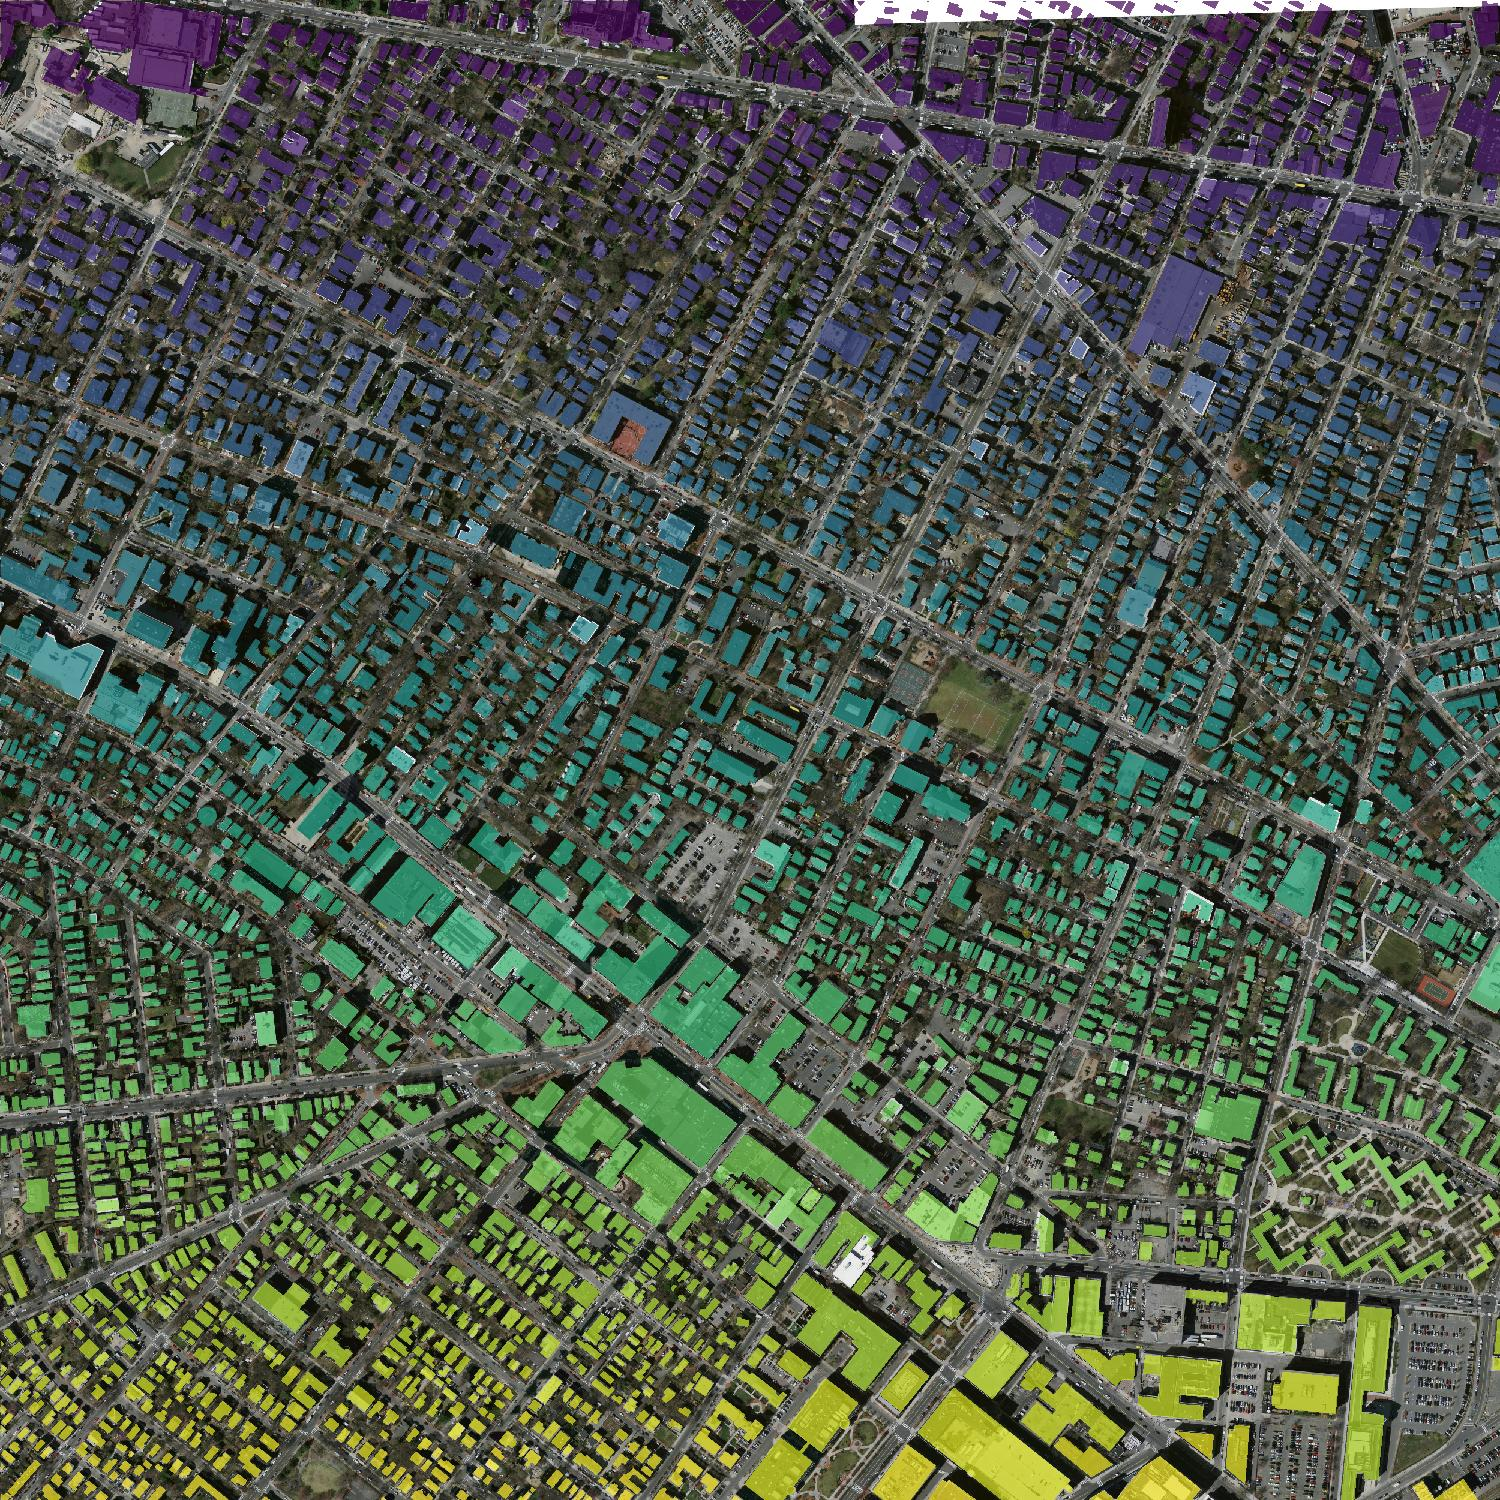
\includegraphics[width=0.25\linewidth]{figures/labelById}%
    }
    \hspace{1em}
    \subfloat[Example using component class as a coloring label]{%
        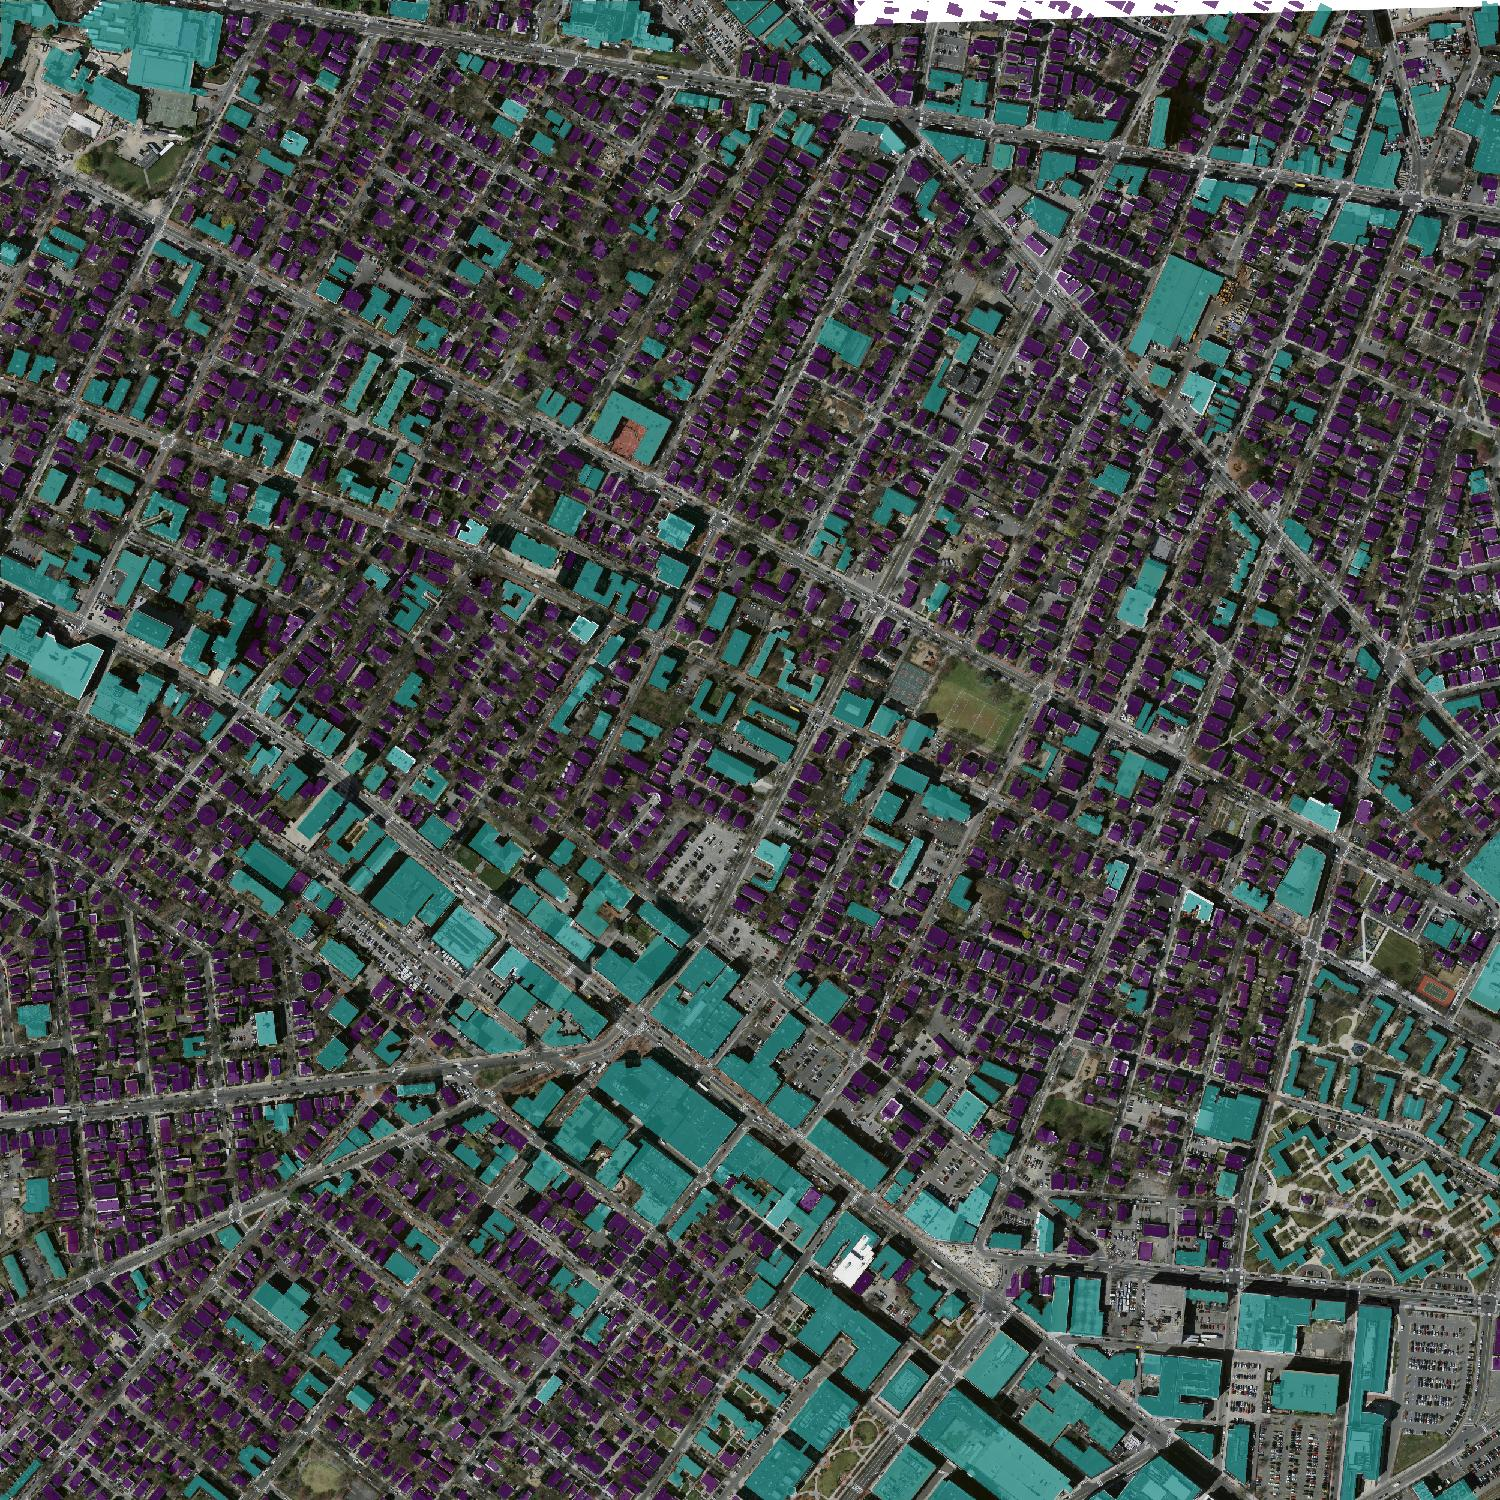
\includegraphics[width=0.25\linewidth]{figures/labelByClass}%
    }
    \hspace{1em}
    \subfloat[Example using an alternative colormap]{%
        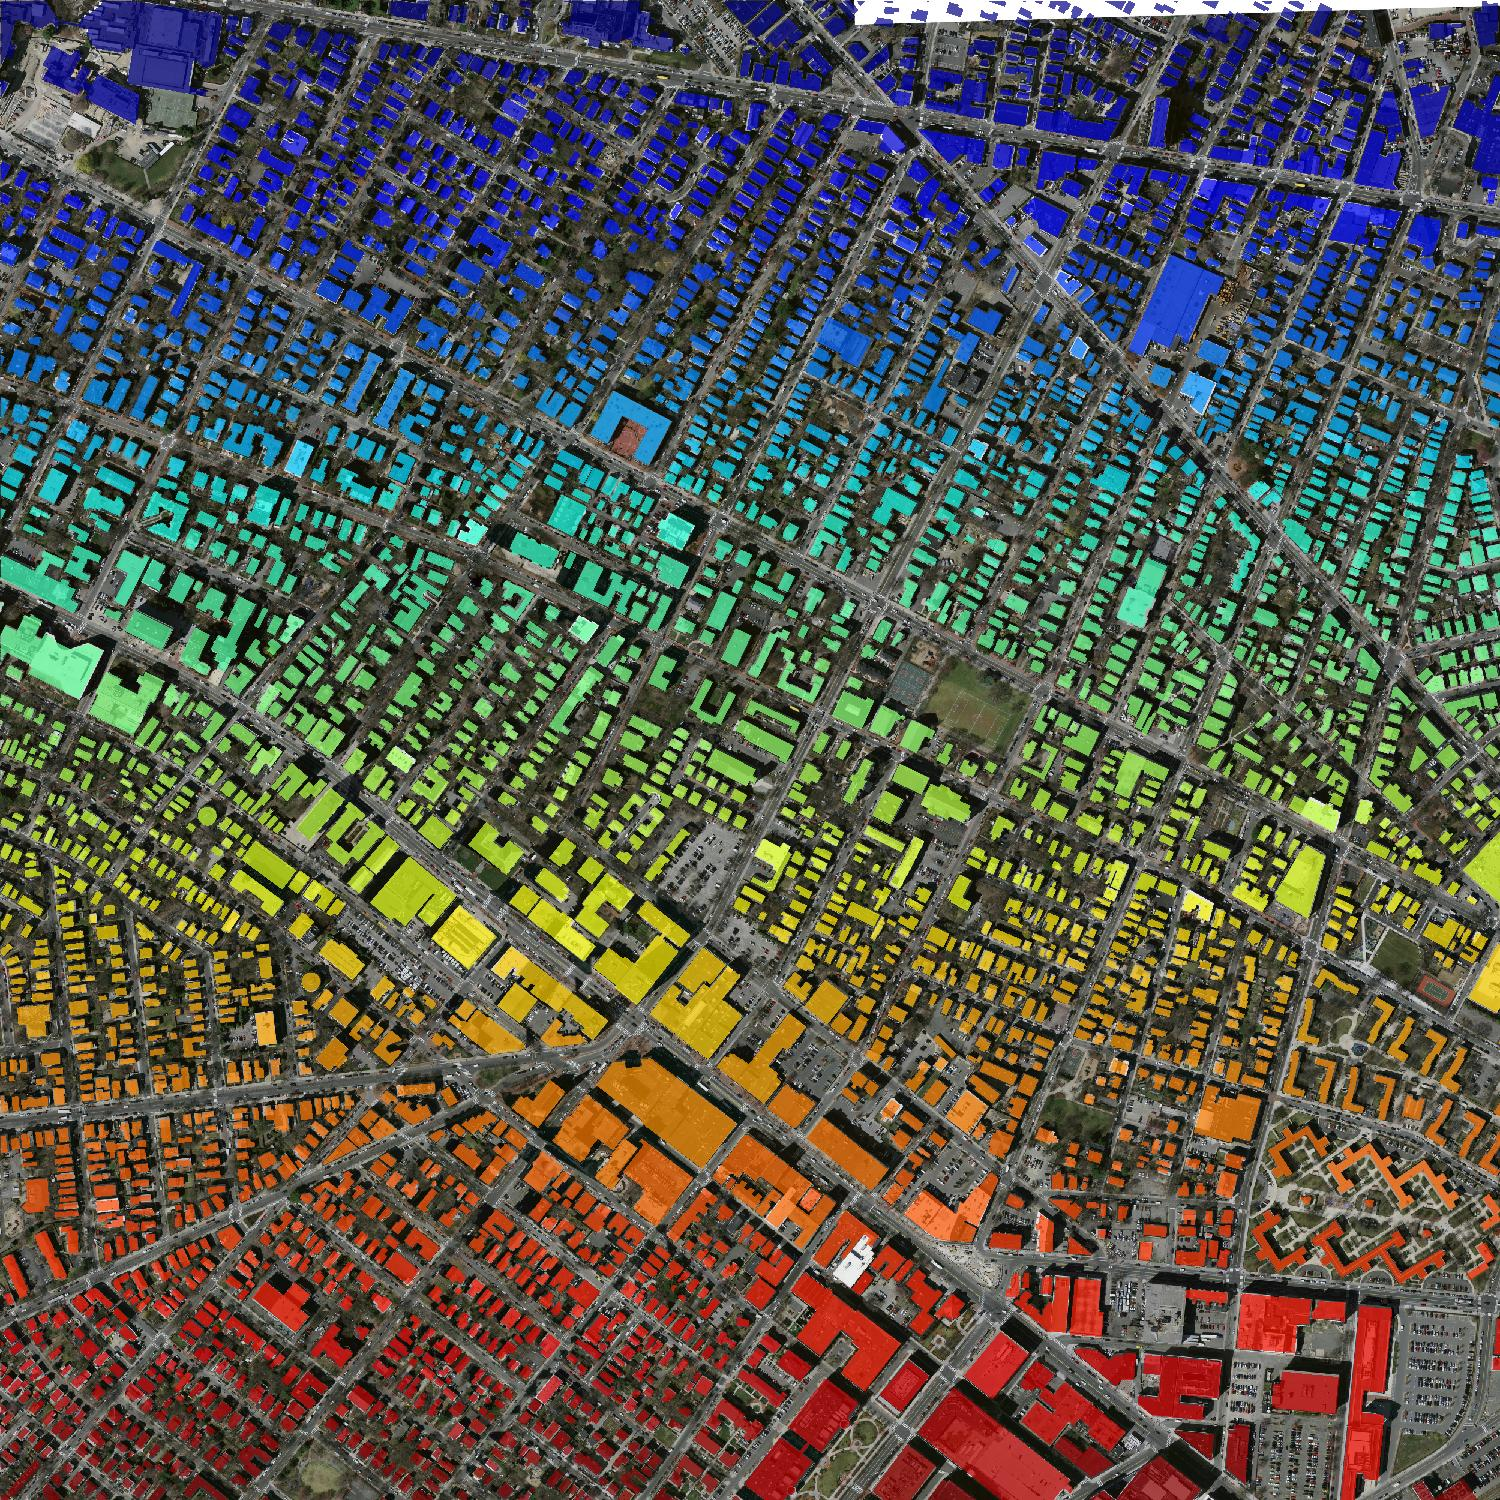
\includegraphics[width=0.25\linewidth]{figures/changeLabelColormap}%
    }
    \hfill
    \caption{Several exports of the same data illustrating the various labeling capabilities within S3A. Arbitrary data columns and arbitrary colormaps may be used.}
    \label{fig:reconfig}
\end{figure*}
}

\newcommand{\makeProcessIllustrationFig}{%
\begin{figure}[!htbp]
    \centering
    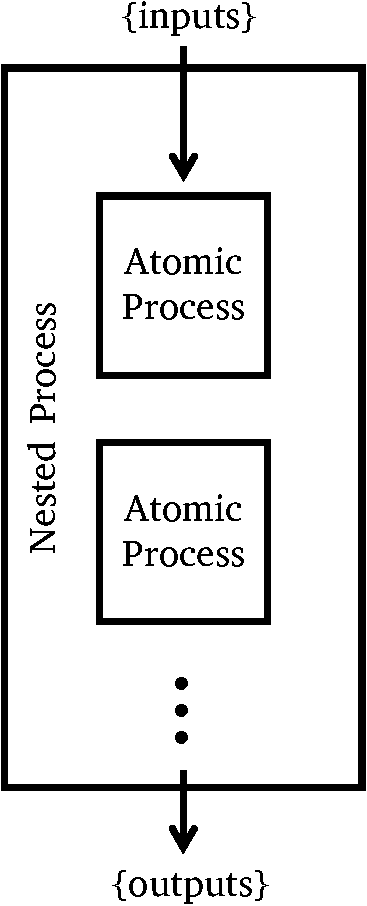
\includegraphics[width=0.3\linewidth]{figures/processIllustration}
    \caption{Depiction of the underlying processing framework. Atomic processes directly wrap functions, and nested processes can contain arbitrary groupings of atomic or nested processes.}
    \label{fig:processIllustration}
\end{figure}
}


\newcommand{\makeAtomicProcFig}{%
\begin{figure*}[!htbp]
    \centering
    \subfloat[Listing for sample outputs]{%
        \RecustomVerbatimEnvironment{Verbatim}{BVerbatim}{}
        \inputminted{Python}{figures/atomicListing.txt}
    }
    \hfill
    \subfloat[Documentation is presented on mouse hover]{%
        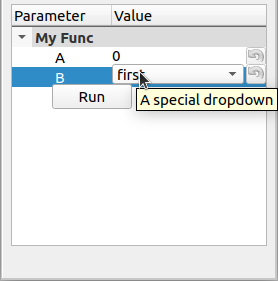
\includegraphics[width=0.29\linewidth]{figures/hoverDoc}%
    }
    \hfill
    \subfloat[GUI constraints are retrieved from specifications]{%
        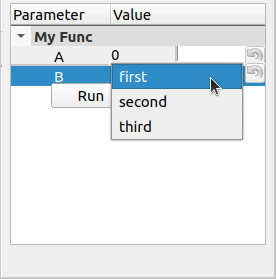
\includegraphics[width=0.29\linewidth]{figures/dropdown}%
    }
    \caption{Several exports of the same data illustrating the various labeling capabilities within S3A. Arbitrary data columns and arbitrary colormaps may be used.}
    \label{fig:atomicProc}
\end{figure*}
}

\newcommand{\makeNestedProcFig}{%
\begin{figure}[!htbp]
    \centering
    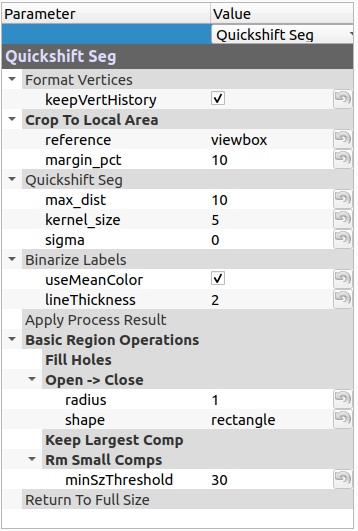
\includegraphics[width=0.5\linewidth]{figures/nestedProc}
    \caption{Processes within S3A can be grouped hierarchically and chained arbitrarily to provide an effective image processing workflow.}
    \label{fig:nestedProc}
\end{figure}
}

\newcommand{\makeAppOverviewFig}{%
\begin{figure*}[!htbp]
    \centering
    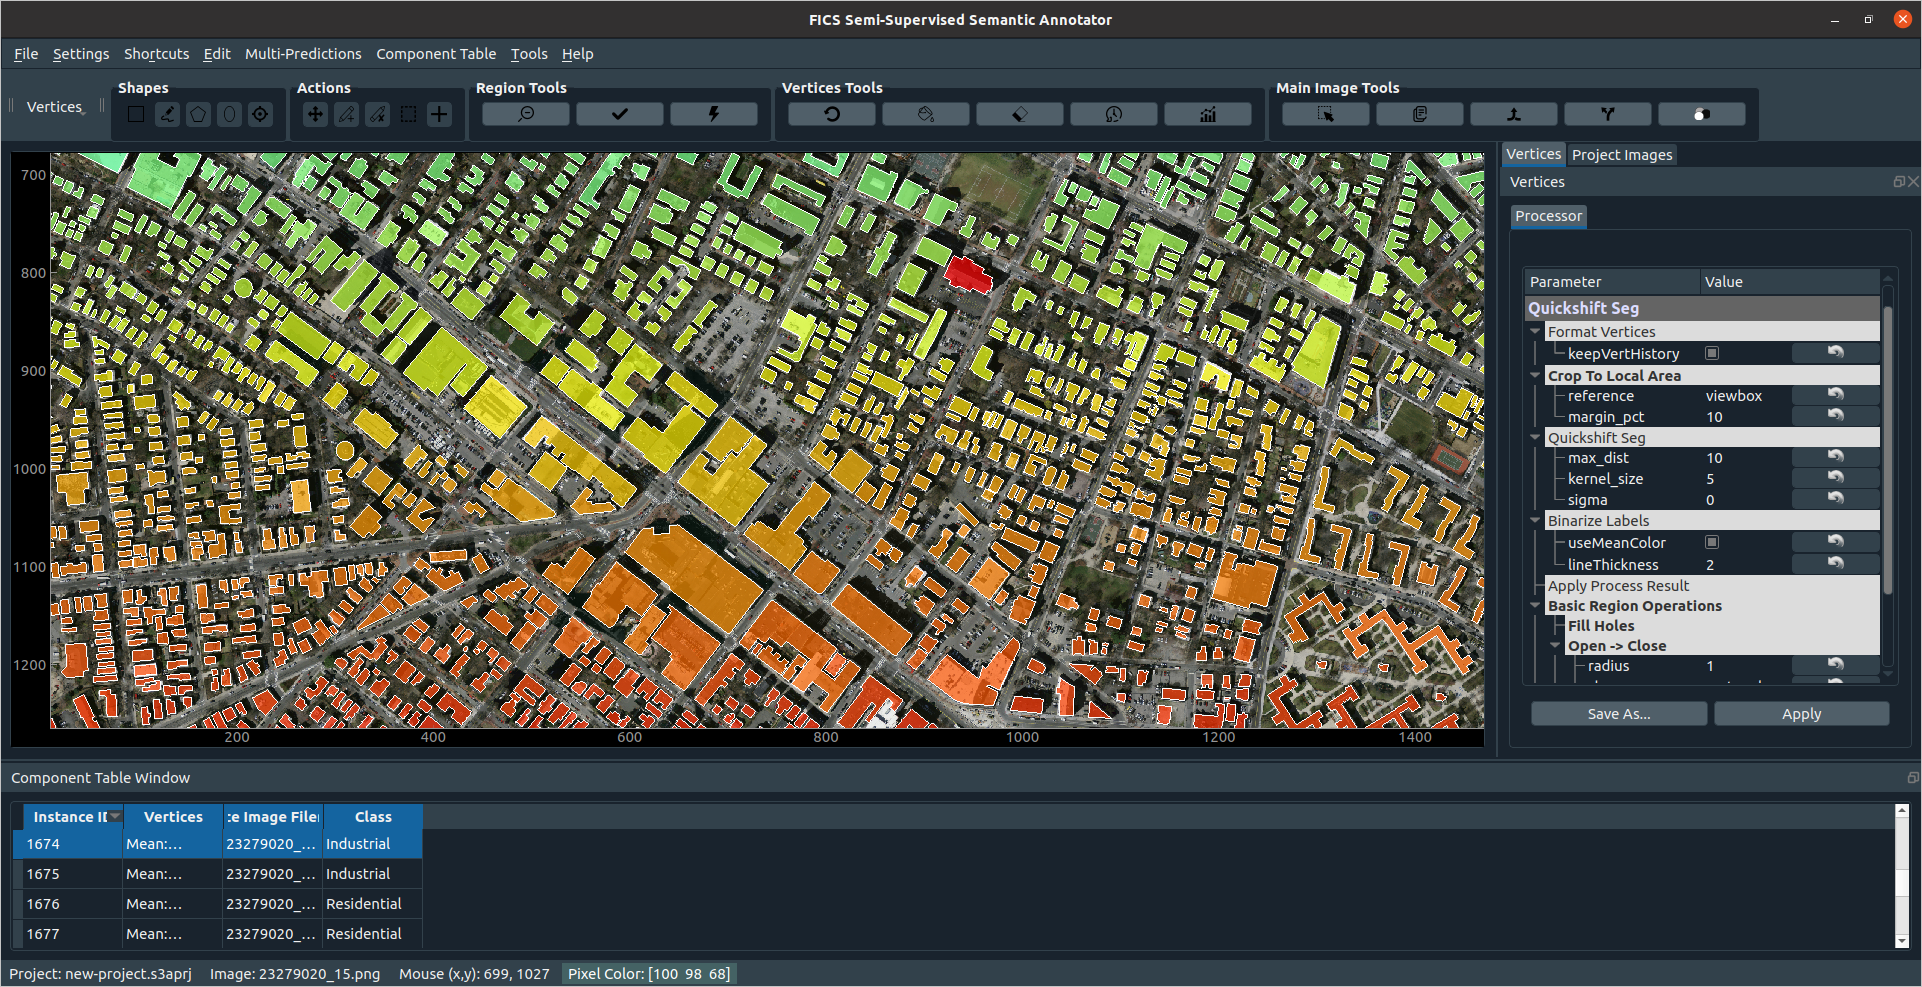
\includegraphics[width=\linewidth]{figures/appOverview}
    \caption{S3A's interface. The main view consists of an image to annotate, a component table of prior annotations, and a toolbar which changes functionality depending on context.}
    \label{fig:appOverview}
\end{figure*}
}
